\documentclass{article}%standalone can be used
\usepackage[utf8]{inputenc}
\usepackage{tikz}
\usetikzlibrary{shapes.geometric, arrows, positioning}

\tikzset{
	startstop/.style = {draw, rectangle, rounded corners, minimum width=3cm, minimum height=1cm, text centered, draw=black, fill=red!30},
	process/.style   = {draw, rectangle, minimum width=3cm, minimum height=1cm, text centered, text width=3cm, draw=black, fill=orange!30},
	decision/.style  = {draw, diamond, minimum width=3cm, minimum height=1cm, text centered, draw=black, aspect=2, fill=green!30},
	arrow/.style     = {->, >=stealth', shorten >=1pt},
	point/.style     = {coordinate}
}

\begin{document}
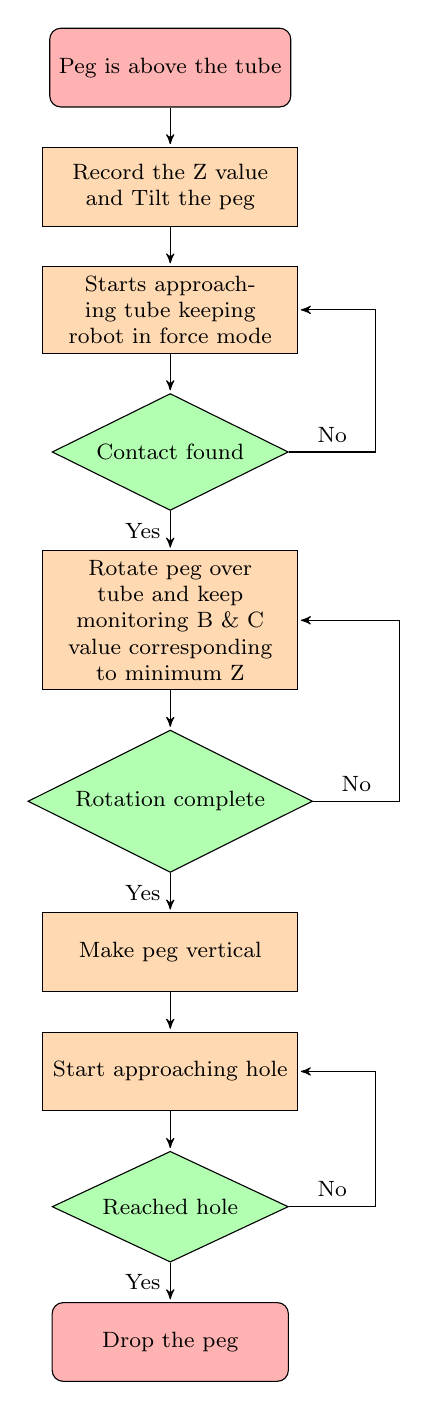
\begin{tikzpicture}[node distance=5mm, every node/.style={font=\footnotesize}]
	\node (start) [startstop] {Peg is above the tube};
	\node (step1) [process, below=of start] {Record the Z value and Tilt the peg};
	\node (step2) [process, below=of step1] {Starts approaching tube keeping robot in force mode};
	\node (step3) [decision, below=of step2] {Contact found};
	\node (step3a)[point, right=of step3, xshift=6mm] {};
	\node (step4) [process, below=of step3] {Rotate peg over tube and keep monitoring B \& C value corresponding to minimum Z};
	\node (step5) [decision, below=of step4] {Rotation complete};
	\node (step5a)[point, right=of step5, xshift=6mm] {};
	\node (step6) [process, below=of step5] {Make peg vertical};
	\node (step7) [process, below=of step6,] {Start approaching hole};
	\node (step8) [decision, below=of step7] {Reached hole};
	\node (step8a)[point, right=of step8, xshift=6mm] {};
	\node (stop)  [startstop, below=of step8] {Drop the peg};

	\draw [arrow] (start) -- (step1);
	\draw [arrow] (step1) -- (step2);
	\draw [arrow] (step2) -- (step3);
	\draw [arrow] (step3) -- node[anchor=east] {Yes} (step4);
	\draw [-]     (step3) -- node[above]{No}(step3a)coordinate(mid1);
	\draw [arrow] (mid1)  |- (step2);
	\draw [arrow] (step4) -- (step5);
	\draw [arrow] (step5) -- node[anchor=east] {Yes} (step6);
	\draw [-]     (step5) -- node[above]{No}(step5a)coordinate(mid2);
	\draw [arrow] (mid2)  |- (step4);
	\draw [arrow] (step6) -- (step7);
	\draw [arrow] (step7) -- (step8);
	\draw [arrow] (step8) -- node[anchor=east] {Yes} (stop);
	\draw [-]     (step8) -- node[above]{No}(step8a)coordinate(mid3);
	\draw [arrow] (mid3)  |- (step7);
\end{tikzpicture}
\end{document}
